\documentclass{llncs}


\usepackage{amsmath} 
\usepackage{bm}
\usepackage{amsbsy} 
\usepackage{amssymb}
\usepackage{cite}
\usepackage{graphicx}

\newcommand{\grad}{\mathop{\rm grad}\nolimits}
\newcommand{\const}{\mathop{\rm const}\nolimits}
\renewcommand{\div}{\mathop{\rm div}\nolimits}
\newcommand{\half}{\frac{1}{2}}

\title{Algorithms for Numerical Simulation of Non-stationary Neutron Diffusion Problems}

\author{A.V. Avvakumov$^{1}$, V.F. Strizhov$^{2}$, P.N. Vabishchevich$^{2}$, A.O. Vasilev$^{3}$ }

\institute{$^1$National Research Center \emph{Kurchatov Institute}, Moscow, Russia \\
$^2$Nuclear Safety Institute of RAS,  Moscow, Russia \\
$^3$North-Eastern Federal University, Yakutsk, Russia}

\begin{document}

\maketitle

\begin{abstract}
The paper is devoted to the issues of modelling the reactor dynamics using multi-group neutron diffusion approximation. Two schemes for the time approximation were considered, namely, an implicit and an explicit-implicit one. For the numerical solution a finite element software was developed based on the package FEniCS and the spectral problems library SLEPc. The code Gmsh is used for the mesh generation. Numerical tests were performed to analyse a regular mode of the VVER-type reactor model.

\end{abstract}


\section{Introduction}
\label{s-1}
The physical processes occuring in a nuclear reactor, depend on the distribution of neutron flux, a mathematical description of which is based on neutron transport equation \cite{stacey}. This equation is integro-differential and the neutron flux distribution is a function of time, energy, spatial and angular variables. For practical use simplifed forms of the equation are usually used in nuclear reactor calculations. The multi-group diffusion approximation \cite{sutton1996diffusion} is most widely used to analyze the reactor. This approach is used in the majority of engineering neutronic codes. 

Engineering neutronic codes are developed to model neutron transport in the multi-group diffusion approximation using, as a rule, finite-difference schemes for space variables.
The diffusion equation solution is the energy-space distribution of neutron flux (including effective multiplication factor for steady-state calculation). The calculated neutronics parameters are, as a matter of fact, functionals of neutron flux density. 

To increase calculational accuracy, nodal methods are widely used
(see, for instance, \cite{lawrence1986progress}). These methods allow modelling on a rather coarse mesh (only a few points per assembly in plane and several tens of axial layers).
The basic idea of a nodal method is to represent neutron flux within a calculational cell as a few-degree polynomial function or as a set of 1-D or 2-D functions. Nodal methods can be connected, in some respect, to the special variants of finite-element approximation \cite{grossman2007nodal}. We can note that it is more appropriate to use the standard procedures of increasing accuracy of the finite-element approximation for boundary problem solution with mesh refinement and using high-order finite elements.

After the discretization of the neutron flux equation, we get a set of linear algebraic equations which is solved iteratively. To obtain suitable calculational accuracy for a boundary problem of a set of diffusion equations, it is necessary to use a rather fine calculational mesh (about several tens of points per assembly in plane and so many axial layers) that leads to increasing calculational time.

To model reactor dynamics, the standard methods to obtain approximate non-stationary solution are used \cite{sutton1996diffusion,stacey}. The most attention should be payed to two-level weighted schemes ($\theta$-method) \cite{Ascher2008}, also the Runge-Kutta and Rosenbrok schemes are used \cite{HairerWanner2010}. Note a special class of methods for modelling non-stationary neutron transport within the multi-group diffusion approach.
It is based on multiplicative performance of the solution as space-time factorization or quasi-static method \cite{goluoglu2001time}. An approximate solution is defined as a product of two functions, i.e., one of which depends on time and is connected with an amplitude,
another describes space distribution (the shape function). At such approach it is difficult to control approximate solution accuracy, in particular, while calculating complicated neutron flux dynamics.

To characterize the reactor dynamic nature, a spectral parameter $\alpha$ is used.
It is defined as the fundamental eigenvalue of the spectral problem (time-eigenvalue or $\alpha$-eigenvalue problem), related to non-stationary diffusion equations 
\cite{Bell1970,verdu20103d}. Analogously to ordinary problems of heat transfer (see, for example, \cite{luikov2012analytical}) we can define a regular reactor mode.
At large times a neutron flux behaviour is asymptotic. Then we can state space-time factorization of the solution with $\exp(\alpha t)$, as amplitude, and the shape function as the eigenfunction of the spectral problem. 

We studied appearance of the regular mode of neutron flux on the example of modelling a two-group water-type reactor test problem. We represented two schemes with explicit and implicit approximations of terms related to neutron generation.
 
 
\section{Problem definition}

Let's consider modelling neutron flux in a multi-group diffusion approximation. Neutron flux dynamics is considered within limited 2D or 3D domain  $\Omega$ ($\bm x = \{x_1, ..., x_d\} \in \Omega, \ d = 2,3$) with a convex boundary $\partial \Omega$. Neutron transport is described by the set of equations without taking into account delayed neutron source:
 \begin{equation}\label{1}
\begin{split}
 \frac{1}{v_g} \frac{\partial \phi_g}{\partial t} - & \nabla \cdot D_g \nabla \phi_g + \Sigma_g \phi_g 
 - \sum_{g\neq g'=1}^{G} \Sigma_{s,g'\rightarrow g} \phi_{g'} \\
 =  & \ \chi_g \sum_{g'=1}^{G} \nu \Sigma_{fg'} \phi_{g'} , \quad 
 g = 1,2, ..., G .
\end{split}
\end{equation} 
Here $\phi_g(\bm x,t)$ is the neutron flux in group $g$ at point $\bm x$ at time moment $t$,
$G$ is the number of energy groups,
$v_g$ is the effective neutron velocity of group $g$,
$D_g(\bm x)$ is the diffusion coefficient, $\Sigma_g(\bm x,t)$ is the absorption cross-section,
$\Sigma_{s,g'\rightarrow g}(\bm x,t)$ is the cross-section for scattering a neutron from group $g'$ to group $g$,
 $\chi_g$  is the fraction of the of the fission neutrons in group $g$, 
$\nu\Sigma_{fg}(\bm x,t)$ is the generation cross-section in group $g$.\\
The albedo-type conditions are set at the boundary $\partial \Omega$ :
\begin{equation}\label{2}
 D_g\frac{\partial \Phi_g}{\partial n} + \gamma_g \Phi_g = 0, \quad 
 \quad g = 1,2, ..., G ,
\end{equation}
where $n$ is the outer normal to the boundary $\partial \Omega$.
Let's consider the problem for equation (\ref{1}) with boundary conditions (\ref{2}), and initial conditions:
\begin{equation}\label{3}
 \phi_g(\bm x,0) = \phi_g^0(\bm x), 
  \quad  g = 1,2, ..., G .
\end{equation} 

Let's write the boundary problem (\ref{1}), (\ref{2}), (\ref{3}) in operator notation. 
We define the vector $\bm \phi = \{\phi_1, \phi_2, ..., \phi_G\}$ and the matrices
\[
 V = (v_{g g'}),
 \quad v_{g g'} = \delta_{g g'} v_g^{-1},
\] 
\[
 D = (d_{g g'}),
 \quad d_{g g'} = - \delta_{g g'} \nabla \cdot D_g \nabla,
\] 
\[
 S = (s_{g g'}),
 \quad  s_{g g'} =  \delta_{g g'} \Sigma_g - \Sigma_{s,g'\rightarrow g} ,
\] 
\[
 R = (r_{g g'}),
 \quad  r_{g g'} = \chi_g \nu \Sigma_{fg'} ,
 \quad g, g' = 1,2, ..., G,
\] 
where
\[
 \delta_{g g'} = \left \{ 
 \begin{matrix}
 1, & g = g', \\
 0, & g \neq  g',
 \end{matrix}
 \right . 
\] 
is the Kronecker delta. We shall use the set of vectors $\bm \phi$,  whose components satisfy the boundary conditions
(\ref{3}). Using introduced definitions, the system of equations (\ref{1}) can be written in the form of the first-order evolutionary equation:
\begin{equation}\label{4}
 V \frac{d \bm \phi}{d t} + (D+S) \bm \phi = R \bm \phi .
\end{equation}  
The Cauchy problem is solved for (\ref{4}), when
\begin{equation}\label{5}
 \bm \phi(0) = \bm \phi^0,
\end{equation} 
where $\bm \phi^0 = \{ \phi_1^0,  \phi_2^0, ...,  \phi_G^0 \}$.

\section{Problem Discretization}

Space discretization is performed using the standard Lagrange finite elements \cite{brenner}. Some details are discussed below while considering the test problem.
 
To perform time approximation, let's consider two schemes: the fully implicit and explicit-implicit ones. Let's $\tau$ is the step of even time mesh, that is $\bm\phi^{n}=\bm\phi(\bm x,t_n)$, where $t_n=n\tau$, $n=0,1,...,N$, $N\tau=T$.  
We consider the fully implicit scheme of first order \cite{Samarskii} as the basic one to obtain an approximate solution of the problem (\ref{4}), (\ref{5}). In this case 
\begin{equation}\label{6}
 V\frac{\bm\phi^{n+1}-\bm\phi^n}{\tau}+(D+S)\bm\phi^{n+1} = R \bm\phi^{n+1},
\end{equation} 
at the known $\bm\phi^{0}$.
At new time level the following problem is to be solved:
\begin{equation}\label{7}
  A \bm\phi^{n+1} = \bm b,
\end{equation} 
where
\[
 A = \frac{V}{\tau}+D+S-R , 
 \quad  \bm b = \frac{V}{\tau}\bm\phi^n.
\]

To move to new time level we should solve a set of coupled elliptic equations of second order. We can use a decoupled scheme which takes into account the solution
features of the non-stationary neutron problems. The operator-matrices $V, D$ are diagonal, and $S$  --- lower triangular matrix.
Coupling of the equations is due to only the operator-matrix of neutron generation $R$.
For this reason the explicit-implicit scheme has evident calculational prospects:
\begin{equation}\label{8}
 V\frac{\bm\phi^{n+1}-\bm\phi^n}{\tau}+(D+S)\bm\phi^{n+1} = R \bm\phi^{n}.
\end{equation} 
This scheme leads to problem (\ref{7}) with
\[
 A = \frac{V}{\tau}+D+S, 
 \quad \bm b = \left(\frac{V}{\tau}+R\right)\bm\phi^n.
\]
While using the explicit-implicit scheme (\ref{8}) we have separate independent sub-problems for neutrons of separate groups.

\section{Test problem}

The test problem for reactor VVER-1000 without a reflector in a two-dimensional approximation ($\Omega$ --- is the reactor core area) is considered \cite{chao}. The geometrical model of the VVER-1000 reactor core consists of a set of hexagonal assemblies and is presented in Fig.\ref{fig:1}, where assemblies of various
types are marked with various numbers. The fuel assembly pitch equals 23.6 cm. Diffusion neutronics constants in the common notations
are given in Table \ref{t-1}. 
The boundary conditions (\ref{3}) are used at $\gamma_g = 0.5, \ g = 1,2$. The problem is solved at $v_1 = 12, 500, 000$ и  $v_2 = 250, 000$.

\begin{figure}[htp]
  \begin{center}
    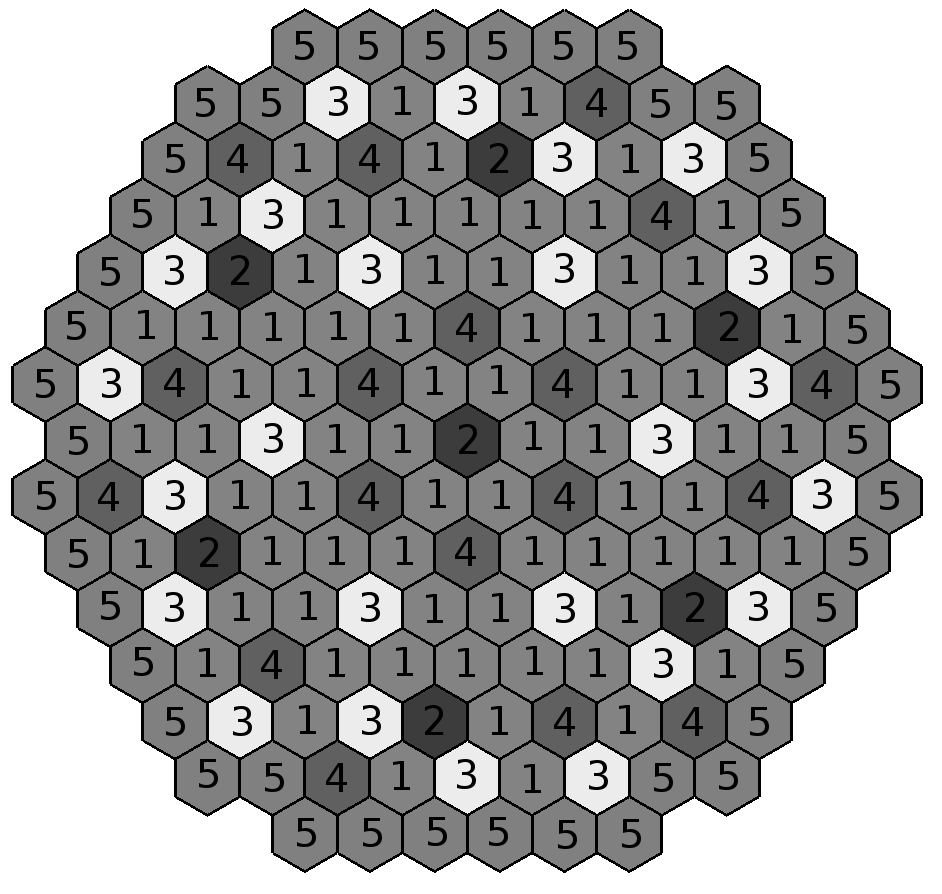
\includegraphics[width=0.5\linewidth] {1.png}
	\caption{Geometrcial model of the VVER-1000 reactor core}
	\label{fig:1}
  \end{center}
\end{figure} 

\begin{table}[htp]
\caption{Diffusion neutronics constants for VVER-1000 test problem}
\label{t-1}
\begin{center}
\begin{tabular}{|c|c|c|c|c|c|}
\hline
Material & 1 & 2 & 3 & 4 & 5\\
\hline
$D_1$ & 1.38320e-0 & 1.38299e-0  & 1.39522e-0  & 1.39446e-0  & 1.39506e-0 \\
$D_2$ & 3.86277e-1 & 3.89403e-1 & 3.86225e-1 & 3.87723e-1 & 3.84492e-1 \\
$\Sigma_1 + \Sigma_{s,1\rightarrow 2}$ & 2.48836e-2 & 2.62865e-2 & 2.45662e-2 & 2.60117e-2 & 2.46141e-2\\
$\Sigma_2$ & 6.73049e-2 & 8.10328e-2 & 8.44801e-1 & 9.89671e-2 & 8.93878e-2\\
$\Sigma_{s,1\rightarrow 2}$ & 1.64977e-2 & 1.47315e-2 & 1.56219e-2 & 1.40185e-2 & 1.54981e-2\\
$\nu\Sigma_{f1}$ & 4.81619e-3 & 4.66953e-3 & 6.04889e-3 & 5.91507e-3 & 6.40256e-3\\
$\nu\Sigma_{f2}$ & 8.46154e-2 & 8.52264e-2 & 1.19428e-1 & 1.20497e-1 & 1.29281e-1\\
\hline
\end{tabular}
\end{center}
\end{table}

To obtain approximate solutions we use the finite element methods \cite{brenner} 
with a triangular calculational mesh. The number of triangles per one assembly $\kappa$  varies from 6 to 96. The standard Lagrangian finite elements of degree $p=1,2,3$ are used. 
The software has been developed using the engineering and scientific calculation library FEniCS \cite{fenics}. The SLEPc package \cite{slepc} has been used for numerical solution of the spectral problems.
 
Let's consider the solution of the spectral problem, called Lambda Modes problem:
\begin{equation}\label{9}
 A \bm \varphi  =  \lambda^{(\alpha)} V \bm \varphi ,
 \quad A = D + S - R . 
\end{equation} 
The fundamental eigenvalue
\[ 
 \alpha = \lambda^{(\alpha)}_1
\]
is called $\alpha$--eigenvalues or period eigenvalues. The asymptotic behaviour (at large times) of the solution of Cauchy problem  (\ref{4}), (\ref{5}) can be connected with the $\alpha$--eigenvalue. In this regular mode, the reactor behaviour is described by the function $e^{-\alpha t} \varphi_{\alpha}(\bm{x})$. 

In the framework of used two-group model, the spectral problem (\ref{9}) can be written as:
\begin{equation}\label{10}
\begin{split}
 - \nabla \cdot D_1 \nabla \varphi_1 & + \Sigma_1 \varphi_1 + \Sigma_{s,1\rightarrow 2} \varphi_1  
 - (\nu \Sigma_{f1} \varphi_1 + \nu \Sigma_{f2} \varphi_2) = \lambda^{(\alpha)} \frac{1}{v_1}   \varphi_1, \\
 - \nabla \cdot D_2 \nabla \varphi_2 & + \Sigma_2 \varphi_2 - \Sigma_{s,1\rightarrow 2} \varphi_1  
 = \lambda^{(\alpha)} \frac{1}{v_2}   \varphi_2.
\end{split}
\end{equation} 
The aim is to define the fundamental eigenvalue $\alpha = \lambda_1^{(\alpha)}$: $\lambda_1^{(\alpha)} \leq  \lambda_2^{(\alpha )} \leq ...$. 

The results of solution of the spectral problem (\ref{10}) for the first eigenvalues $\alpha_n = \lambda_n^{(\alpha)}, \ n = 1,2, ..., 5$
using the different grids and finite elements
are shown in Table \ref{t-2}. 
The eigenvalues $\alpha_2, \alpha_3$, $\alpha_4, \alpha_5$, $\alpha_9, \alpha_{10}$ are the complex values with small imaginary parts, and the eigenvalues $\alpha_1, \alpha_6$, $\alpha_7, \alpha_8$ are the real values.

\begin{table}[htp]
\caption{The eigenvalues $\alpha_n = \lambda_n^{(\alpha )}, \ n = 1,2, ..., 5$}
\label{t-2}
\begin{center}
\begin{tabular}{|c|c|c|c|c|}
\hline
$\kappa$ & $p$ & $\alpha_1$ &  $\alpha_2, \alpha_3$ &  $\alpha_4, \alpha_5$ \\ 
\hline
   & 1 & -105.032 & 159.802 $\pm$ 0.025510$i$  & 659.109 $\pm$ 0.034667$i$  \\
6  & 2 & -139.090 & 115.793 $\pm$ 0.029186$i$  & 591.782 $\pm$ 0.034667$i$  \\
   & 3 & -140.223 & 114.035 $\pm$ 0.033814$i$  & 588.762 $\pm$ 0.069025$i$  \\
\hline
   & 1 & -130.422 & 126.984 $\pm$ 0.034409$i$  & 608.734 $\pm$ 0.070724$i$  \\
24 & 2 & -140.187 & 114.089 $\pm$ 0.033512$i$  & 588.849 $\pm$ 0.068555$i$  \\
   & 3 & -140.281 & 113.887 $\pm$ 0.033604$i$  & 588.415 $\pm$ 0.068695$i$  \\
\hline
   & 1 & -137.704 & 117.345 $\pm$ 0.033823$i$  & 593.818 $\pm$ 0.069254$i$  \\
96 & 2 & -140.284 & 113.886 $\pm$ 0.033599$i$  & 588.419 $\pm$ 0.068687$i$  \\
   & 3 & -140.308 & 113.842 $\pm$ 0.033603$i$  & 588.336 $\pm$ 0.068690$i$  \\
\hline
\end{tabular}
\end{center}
\end{table}

The eigenvalues  $\lambda_1^{(\alpha)} \leq  \lambda_2^{(\alpha)} \leq ...$
are well separated. In our example, the fundamental eigenvalue is negative and therefore the main harmonic will increase, while all others will attenuate. The regular mode of the reactor is thereby defined. The value $\alpha = \lambda_1^{(\alpha)}$ determines the amplitude of neutron flux development and connects directly with the reactor period in the regular mode.

The fully implicit (\ref{6}) and explicit-implicit (\ref{8}) schemes are used to define approximate solution at the initial conditions:
\[ 
\phi_1^0 = 1.0, \quad \phi_2^0 = 0.25
\]
and  $k=24$, $p=2$. Let's $T=5\times 10^{-3}$ and consider the fully implicit solution at $\tau = 1 \times 10^{-5}$ as the reference one. 

The appearance of the regular mode of neutron flux is controlled by the proximity of the normed solution of the non-stationary problem 
and the fundamental eigenfunction $\bm \phi$. Let's define for $g=1$:
\[
 \eta(t) = \|\overline{\phi}_1(t) - \overline{\varphi}_1\|, 
 \quad  \overline{\phi}_1(t) = \frac{\phi_1(t)}{\|\phi_1(t)\|} ,
 \quad  \overline{\varphi}_1 = \frac{\varphi_1}{\|\varphi_1\|} .
\] 
The appearance of the dynamic behaviour trend is evaluated by the value:
\[
 \theta(t) = \frac{1}{|\alpha|} \left \| \frac{1}{\phi_1(t)}\frac{\partial \phi_1(t)}{\partial t} - \alpha \right \|.
\] 
Dependence of $\eta(t)$ and $\theta(t)$ on the used time step is shown in Fig.\ref{fig:2} 
for the fully implicit scheme and in Fig.\ref{fig:3} for the explicit-implicit scheme.
The implicit scheme (\ref{6}) has significantly higher accuracy compared to the explicit-implicit scheme (\ref{8}).

\begin{figure}[htp]
  \begin{center}
\begin{minipage}{0.49\linewidth}
\center{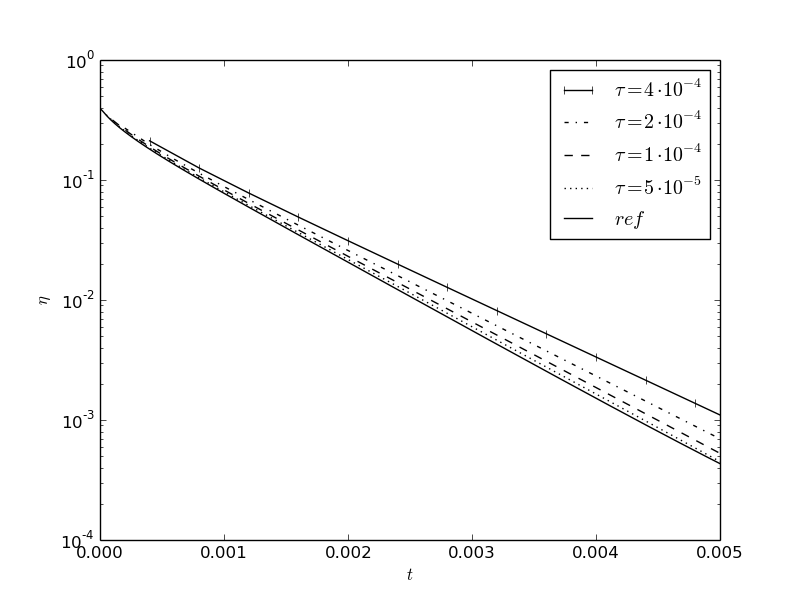
\includegraphics[width=1\linewidth]{2-1.png}} \\
\end{minipage}
\hfill
\begin{minipage}{0.49\linewidth}
\center{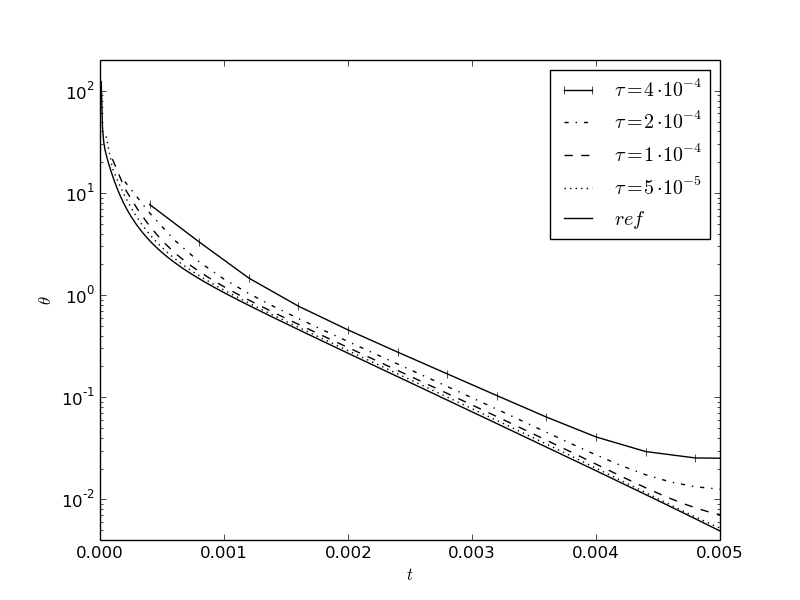
\includegraphics[width=1\linewidth]{2-2.png}} \\
\end{minipage}
\caption{The fully implicit scheme}
\label{fig:2}
  \end{center}
\end{figure}

\begin{figure}[htp]
  \begin{center}
\begin{minipage}{0.49\linewidth}
\center{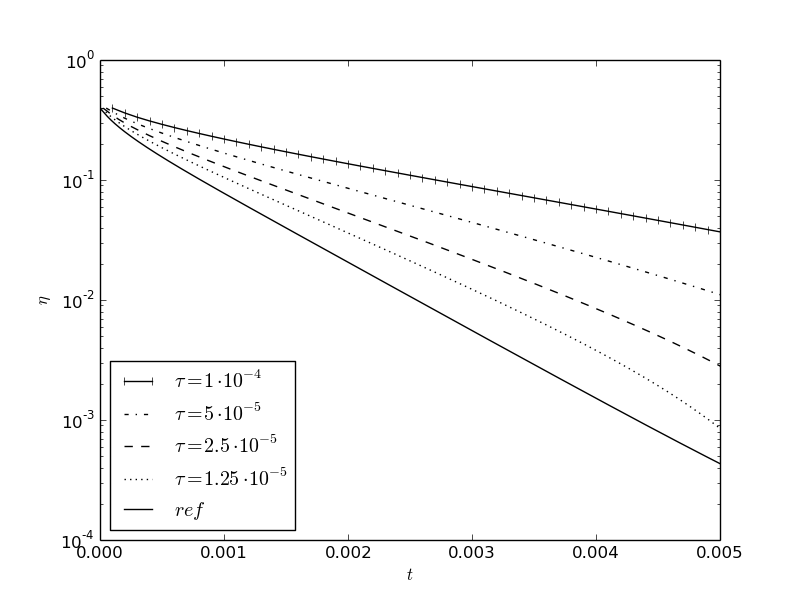
\includegraphics[width=1\linewidth]{3-1.png}} \\
\end{minipage}
\hfill
\begin{minipage}{0.49\linewidth}
\center{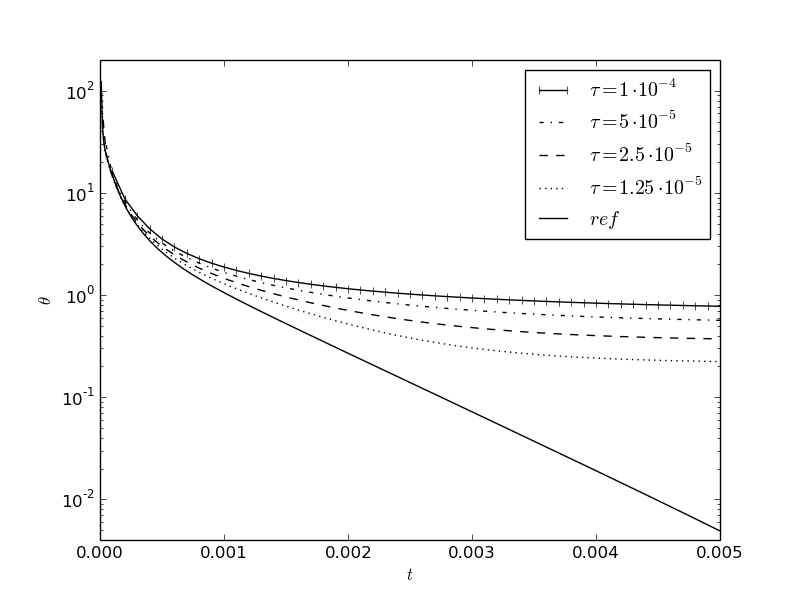
\includegraphics[width=1\linewidth]{3-2.png}} \\
\end{minipage}
\caption{The explicit-implicit scheme}
\label{fig:3}
  \end{center}
\end{figure}

\section*{Acknowledgements}
This work was supported by the Russian Foundation for Basic Research  (projects 16-08-01215).

\begin{thebibliography}{35}
\expandafter\ifx\csname natexlab\endcsname\relax\def\natexlab#1{#1}\fi
\expandafter\ifx\csname url\endcsname\relax
  \def\url#1{\texttt{#1}}\fi
\expandafter\ifx\csname urlprefix\endcsname\relax\def\urlprefix{URL }\fi


\bibitem{Ascher2008}
Ascher, U.M.: Numerical methods for evolutionary differential equations.
  Society for Industrial Mathematics (2008)

\bibitem{Bell1970}
Bell, G.I., Glasstone, S.: Nuclear Reactor Theory. Van Nostrand Reinhold
  Company (1970)

\bibitem{brenner}
Brenner, S.C., Scott, R.: The Mathematical Theory of Finite Element Methods.
  Springer (2008)

\bibitem{slepc}
Campos, C., Roman, J., Romero, E., Tomas, A.: SLEPc Users Manual (2013)

\bibitem{chao}
Chao, Y.A., Shatilla, Y.A.: {Conformal mapping and hexagonal nodal methods-II:
  Implementation in the ANC-H Code}. Nuclear Science and Engineering  121,
  210--225 (1995)

\bibitem{goluoglu2001time}
Goluoglu, S., Dodds, H.L.: A time-dependent, three-dimensional neutron
  transport methodology. Nuclear science and engineering  139(3),  248--261
  (2001)

\bibitem{grossman2007nodal}
Grossman, L.M., Hennart, J.P.: Nodal diffusion methods for space-time neutron
  kinetics. Progress in Nuclear Energy  49(3),  181--216 (2007)

\bibitem{HairerWanner2010}
Hairer, E., Wanner, G.: {Solving ordinary differential equations II: Stiff and
  differential-algebraic problems}. Springer Verlag (2010)

\bibitem{lawrence1986progress}
Lawrence, R.D.: Progress in nodal methods for the solution of the neutron
  diffusion and transport equations. Progress in Nuclear Energy  17(3),
  271--301 (1986)

\bibitem{fenics}
Logg, A., Mardal, K., Wells, G.: Automated Solution of Differential Equations
  by the Finite Element Method: The FEniCS Book. Lecture Notes in Computational
  Science and Engineering, Springer (2012),
  \url{http://books.google.ru/books?id=ASWN\_VRr1NQC}

\bibitem{luikov2012analytical}
Luikov, A.: Analytical Heat Diffusion Theory. Academic Press (1968)

\bibitem{Samarskii}
Samarskii, A.A.: The Theory of Difference Schemes. Marcel Dekker, New York
  (2001)

\bibitem{stacey}
Stacey, W.M.: Nuclear Reactor Physics. Wiley (2007)

\bibitem{sutton1996diffusion}
Sutton, T.M., Aviles, B.N.: Diffusion theory methods for spatial kinetics
  calculations. Progress in nuclear energy  30(2),  119--182 (1996)

\bibitem{verdu20103d}
Verdu, G., Ginestar, D., Roman, J., Vidal, V.: {3D} alpha modes of a nuclear
  power reactor. Journal of Nuclear Science and Technology  47(5),  501--514
  (2010)

\end{thebibliography}
 

\end{document}






